%----------------------1----------------------------------------
\begin{frame}[t]{Resultados y discusión.\\\textit{Entorno de pruebas.}}
\begin{itemize}
    \item Los parámetros de configuración fueron tomados del material bibliográfico de apoyo.
    \item Se generaron aleatoriamente 1.146 larvas para 25 puntos de control.
    \item El periodo de simulación fue de 50 días, a temperatura constante.
    \item La dirección del viento seleccionada fue la suroeste.
    \item Comparar las tasas de desarrollo obtenidas con los resultados obtenidos por expertos en laboratorio.
    \end{itemize}
\end{frame}

\begin{frame}[t]{Resultados y discusión. \textit{Población inicial.}}
    \begin{center}
        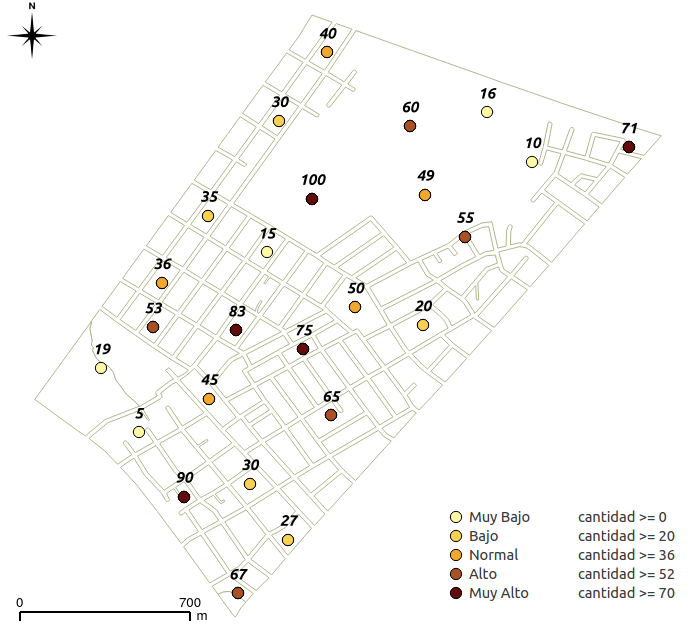
\includegraphics[width=7.5cm]{./graphics/extension-poblacion.png}
    \end{center}
\end{frame}
%--------------------------2------------------------------------

\begin{frame}[t]{Resultados y discusión.\\\textit{Tasas de desarrollo de los huevos.}}
    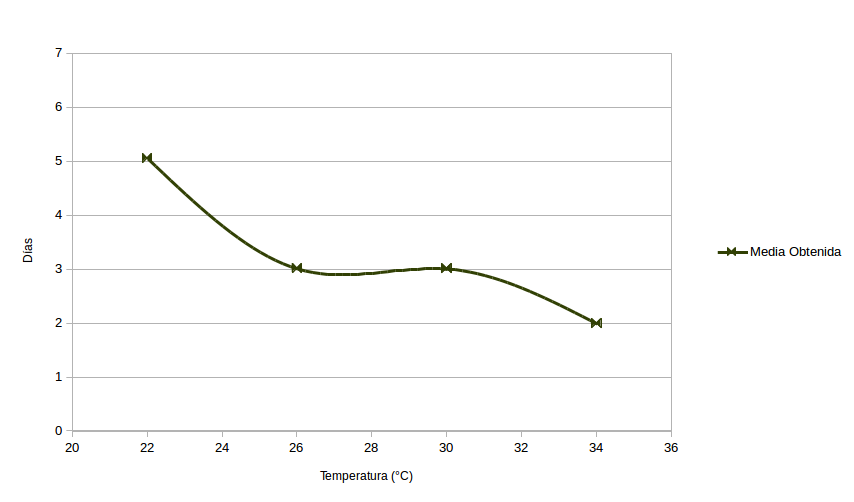
\includegraphics[width=\textwidth]{./graphics/huevos-desarrollo-single.png}
\end{frame}

\begin{frame}[t]{Resultados y discusión.\\\textit{Tasas de desarrollo de los huevos.}}
    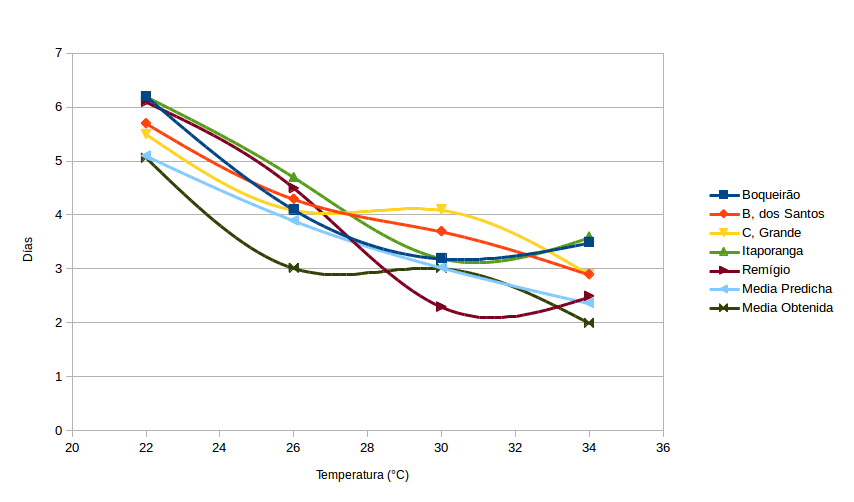
\includegraphics[width=\textwidth]{./graphics/huevos-desarrollo.png}
\end{frame}

\begin{frame}[t]{Resultados y discusión.\\\textit{Tasas de desarrollo de las larvas.}}
    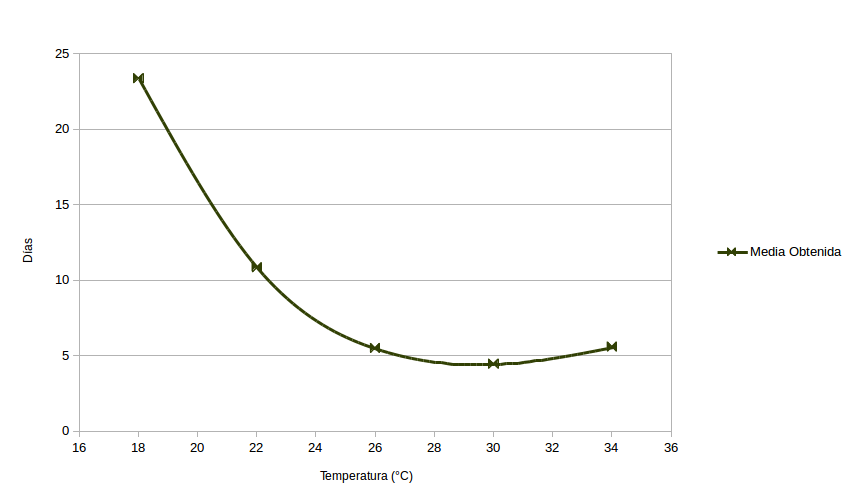
\includegraphics[width=\textwidth]{./graphics/larvas-desarrollo-single.png}
\end{frame}

\begin{frame}[t]{Resultados y discusión.\\\textit{Tasas de desarrollo de las larvas.}}
    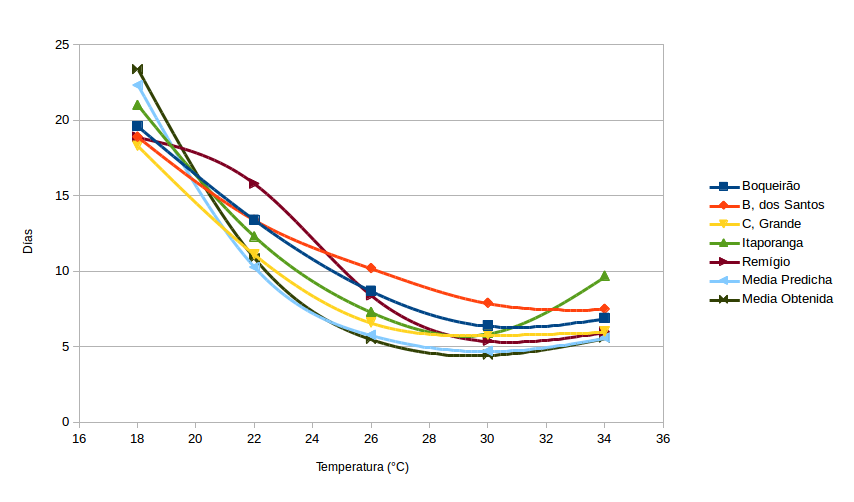
\includegraphics[width=\textwidth]{./graphics/larvas-desarrollo.png}
\end{frame}

\begin{frame}[c]{Resultados y discusión.\\\textit{Tasas de desarrollo de las pupas.}}
    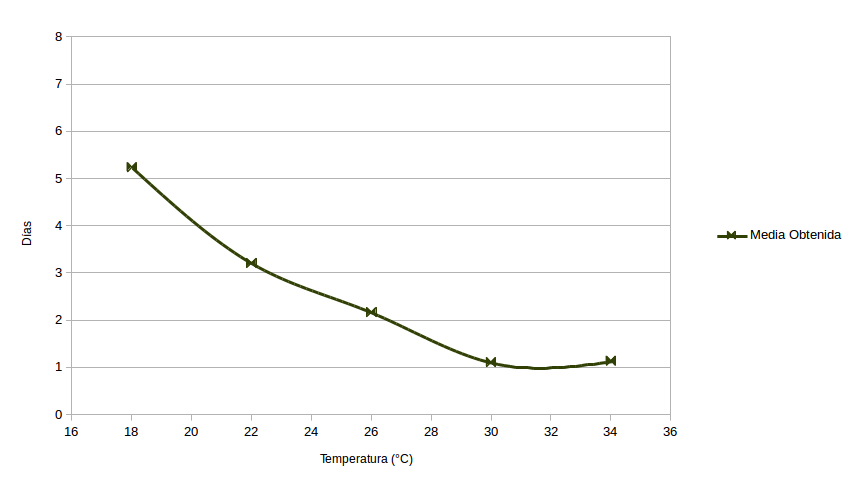
\includegraphics[width=\textwidth]{./graphics/pupas-desarrollo-single.png}
\end{frame}

\begin{frame}[c]{Resultados y discusión.\\\textit{Tasas de desarrollo de las pupas.}}
    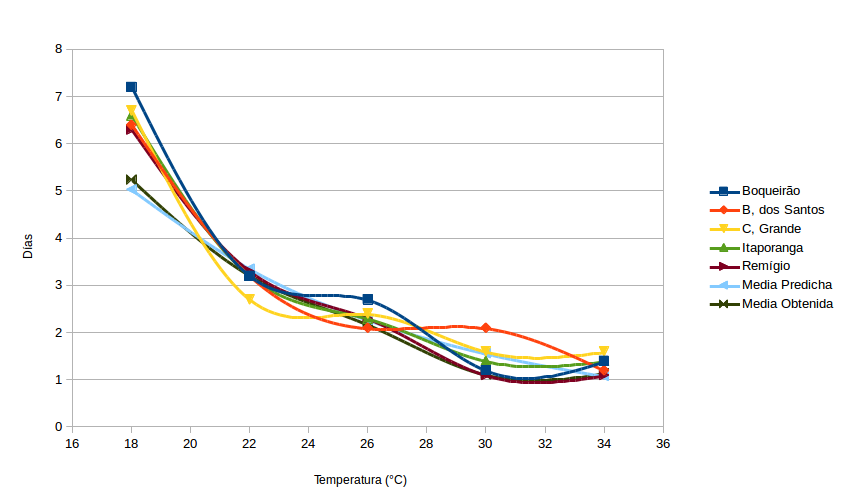
\includegraphics[width=\textwidth]{./graphics/pupas-desarrollo.png}
\end{frame}

\begin{frame}[t]{Resultados y discusión.\\\textit{Ciclo gonotrófico.}}
    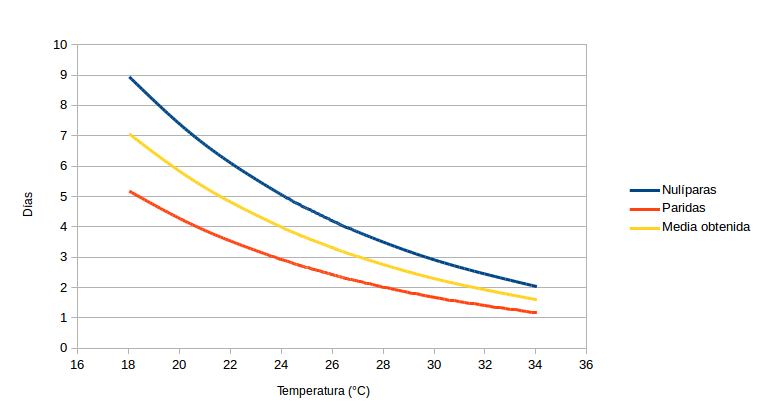
\includegraphics[width=\textwidth]{./graphics/ciclo-gonotrofico-temperatura.png}
\end{frame}

%--------------------------2------------------------------------

\begin{frame}[t]{Resultados y discusión.\\\textit{Crecimiento de la población en etapas inmaduras.}}
\begin{center}
    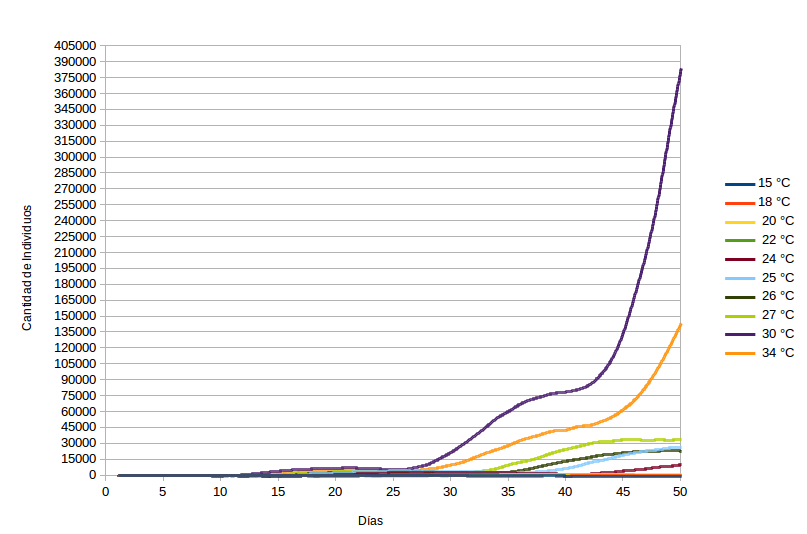
\includegraphics[width=9.3cm]{../paper/graphics/evolucion-poblacion-all.png}
\end{center}
\end{frame}

\begin{frame}[t]{Resultados y discusión.\\\textit{Crecimiento de la población de adultos.}}
\begin{center}
    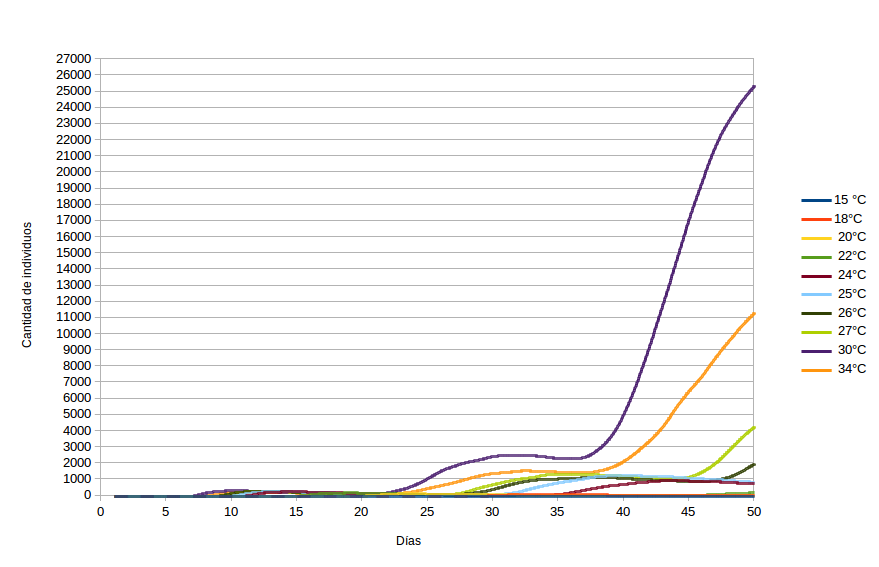
\includegraphics[width=9.3cm]{../paper/graphics/evolucion-poblacion-adultos.png}
\end{center}
\end{frame}

\begin{frame}[t]{Resultados y discusión.\\\textit{Focos de infestación}}
\begin{center}

\begin{table}[!hptb]
    \begin{minipage}{\textwidth}
    \scriptsize
    \centering
    \caption{\label{tab:niveles-riesgo-zonas} Clasificación de los niveles de infestación de acuerdo al tipo de zona.}
    \begin{tabular}{l l c c c}
        \hline\\
         Niveles de infestación & Tipo de zona & Mínimo $u(x,y)$$^a$ & Máximo $u(x,y)$$^a$ \\
        \hline
        \hline
        Muy bajo & Pésima  & 0  & 19 \\
        Bajo     & Mala    & 20 & 35 \\
        Medio    & Regular & 36 & 51 \\
        Alto     & Buena   & 52 & 69 \\
        Muy Alto & Óptima  & 70 & --$^b$\\
    \end{tabular}
    \footnotetext[1]{\scriptsize Rango mínimo y máximo de $u(x,y)$ permitido para el tipo de zona.}
    \footnotetext[2]{\scriptsize No se estableció un límite superior para este nivel. }
    \end{minipage}
\end{table}
\end{center}
\end{frame}

%--------------------------2------------------------------------

\begin{frame}[t]{Resultados y discusión.\\\textit{Mapas de interpolación a 20 \textcelsius.}}
    \begin{figure}
    \begin{subfigure}[b]{0.45\textwidth}
        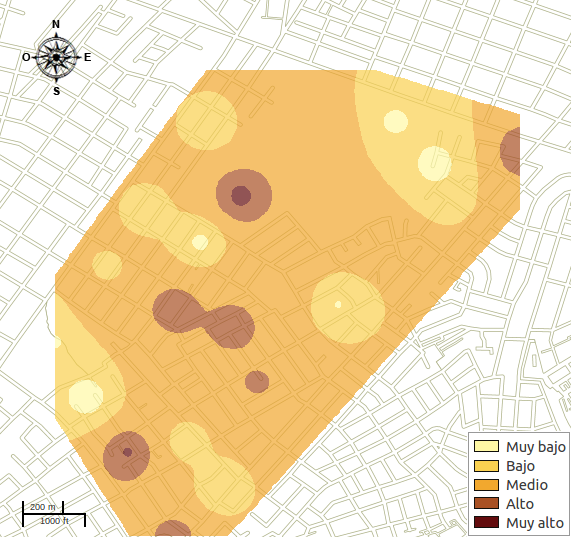
\includegraphics[width=\textwidth]{../book/capitulo-6/graphics/raster/temp-20-0.png}
        \caption{ Primer día de simulación.}
    \end{subfigure}
    ~~~~
    \begin{subfigure}[b]{0.45\textwidth}
        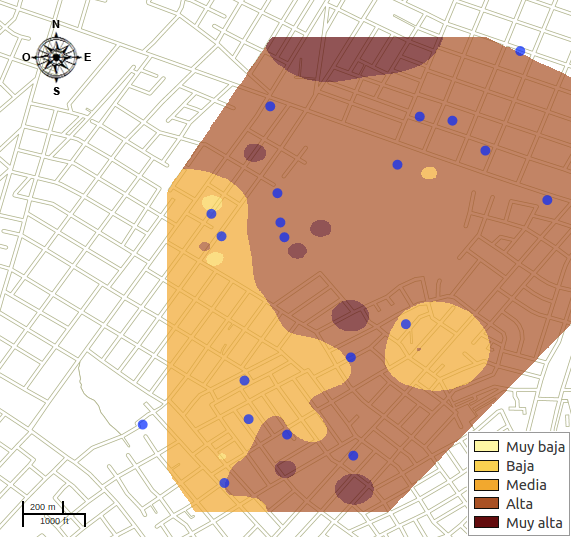
\includegraphics[width=\textwidth]{../book/capitulo-6/graphics/raster/temp-20-38.png}
        \caption{Día número 50 de simulación.}
    \end{subfigure}
    \end{figure}
\end{frame}

\begin{frame}[t]{Resultados y discusión.\\\textit{Mapas de interpolación a 24 \textcelsius.}}
    \begin{figure}
    \begin{subfigure}[b]{0.45\textwidth}
        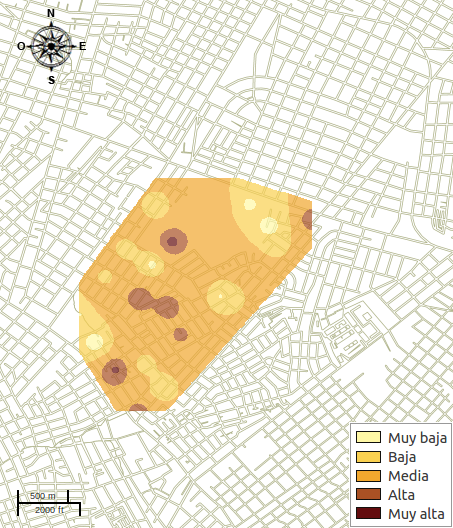
\includegraphics[width=4.5cm]{../book/capitulo-6/graphics/raster/temp-24-0.png}
        \caption{ Primer día de simulación.}
    \end{subfigure}
    ~~~~
    \begin{subfigure}[b]{0.45\textwidth}
        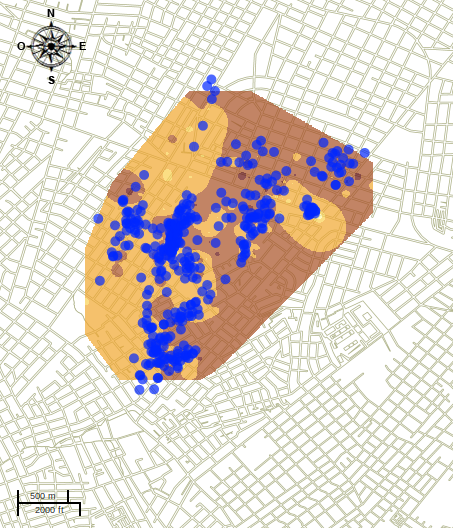
\includegraphics[width=4.5cm]{../book/capitulo-6/graphics/raster/temp-24-49.png}
        \caption{Día número 50 de simulación.}
    \end{subfigure}
    \end{figure}
\end{frame}

\begin{frame}[t]{Resultados y discusión.\\\textit{Mapas de interpolación a 27 \textcelsius.}}
    \begin{figure}
    \begin{subfigure}[b]{0.45\textwidth}
        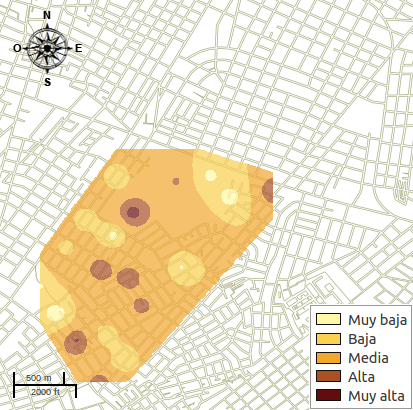
\includegraphics[width=\textwidth]{../book/capitulo-6/graphics/raster/temp-27-0.png}
        \caption{ Primer día de simulación.}
    \end{subfigure}
    ~~~~
    \begin{subfigure}[b]{0.45\textwidth}
        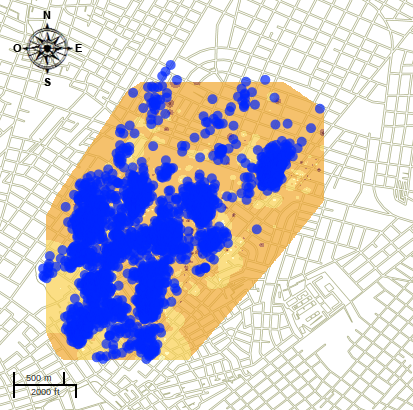
\includegraphics[width=\textwidth]{../book/capitulo-6/graphics/raster/temp-27-49.png}
        \caption{Día número 50 de simulación}
    \end{subfigure}
    \end{figure}
\end{frame}

\begin{frame}[t]{Resultados y discusión.\\\textit{Mapas de interpolación a 30 \textcelsius.}}
    \begin{figure}
    \begin{subfigure}[b]{0.45\textwidth}
        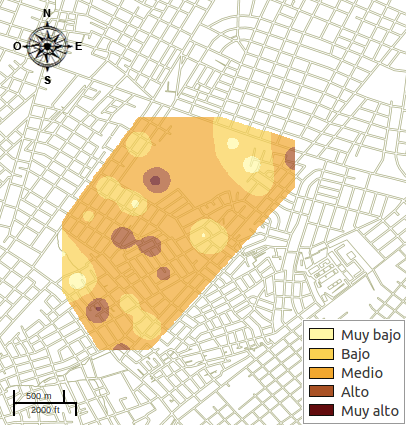
\includegraphics[width=\textwidth]{../book/capitulo-6/graphics/raster/temp-30-0.png}
        \caption{ Primer día de simulación.}
    \end{subfigure}
    ~~~~
    \begin{subfigure}[b]{0.45\textwidth}
        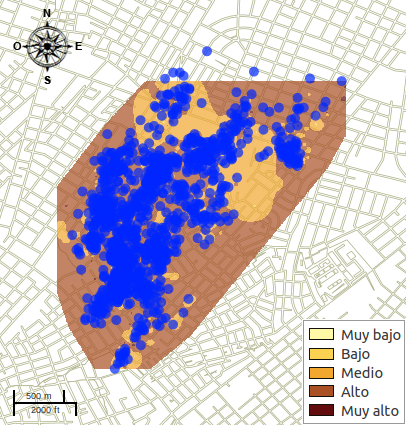
\includegraphics[width=\textwidth]{../book/capitulo-6/graphics/raster/temp-30-35.png}
        \caption{Día número 50 de simulación.}
    \end{subfigure}
    \end{figure}
\end{frame}


\begin{frame}[t]{Resultados y discusión.\\\textit{Mapas de interpolación a 34 \textcelsius.}}
    \begin{figure}
    \begin{subfigure}[b]{0.45\textwidth}
        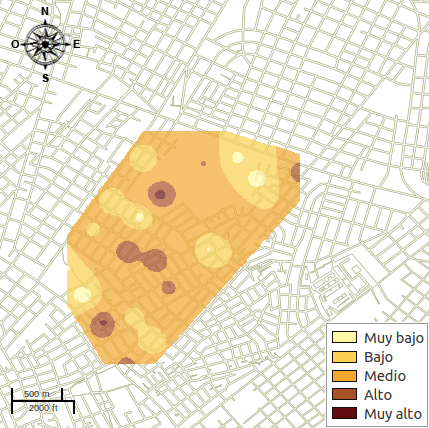
\includegraphics[width=\textwidth]{../book/capitulo-6/graphics/raster/temp-34-0.png}
        \caption{ Primer día de simulación.}
    \end{subfigure}
    ~~~~
    \begin{subfigure}[b]{0.45\textwidth}
        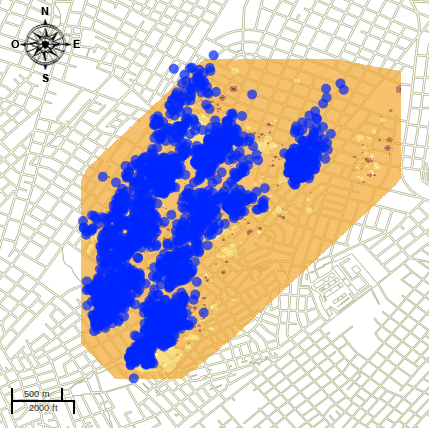
\includegraphics[width=\textwidth]{../book/capitulo-6/graphics/raster/temp-34-42.png}
        \caption{Día número 50 de simulación.}
    \end{subfigure}
    \end{figure}
\end{frame}
